\documentclass{article}
% \documentclass[twocolumn]{article}
\usepackage{graphicx} % Required for inserting images
\usepackage{tikz} 
\usepackage{amsmath}
\usepackage{booktabs}

\newcommand{\mybox}[5]{
    \begin{center}
    \begin{tikzpicture}
        \node[anchor=text,text width=\columnwidth+1.0cm, draw, rounded corners, line width=1pt, fill=#3, inner sep=5mm] (big) {\\#4};
        \node[draw, rounded corners, line width=.5pt, fill=#2, anchor=west, xshift=5mm] (small) at (big.north west) {#1};
    \end{tikzpicture}
    % \caption{#5}
    \end{center}
}



\title{Snarkifying Mithril Discussion}
\author{Wuyunsiqin \quad \quad Bingsheng Zhang \\ 
Zhejiang University, CHN \\
22521299@zju.edu.cn \quad bingsheng@zju.edu.cn}
% \date{May 20 2025}




\begin{document}

\maketitle


\section{Mithril Review}
\subsection{MSP-PoP}

Mithril use a variant of MSP-PoP, a multisignature based on Boneh–Lynn–Shacham (BLS) signatures with proofs of possession (PoPs). Let $q$ be a prime, $\mathbb{G}_1,\mathbb{G}_2,\mathbb{G}_T$ be cyclic groups of order $q$ with generators $g_1\in\mathbb{G}_1$, $g_2\in\mathbb{G}_2$, and bilinear pairing $e:\mathbb{G}_1\times\mathbb{G}_2\to\mathbb{G}_T$. Let $H_{\mathbb{G}_1}:\{0,1\}^\ast\to\mathbb{G}_1$ be a hash-to-$\mathbb{G}_1$ function, $H_\lambda:\{0,1\}^\ast\to\mathbb{Z}_{2^\lambda}$ a short-exponent hash, and $H_p:\{0,1\}^\ast\to\mathbb{F}_p$ a collision-resistant hash.

\begin{itemize}
  \item \textbf{MSP.Gen}$(\mathsf{Param})$: Sample $sk\leftarrow \mathbb{Z}_q$; set $mvk \leftarrow g_2^{sk}$. Compute
  \(
    \kappa_1 \leftarrow H_{\mathbb{G}_1}(\text{``PoP''}\parallel mvk)^{sk},
    \qquad
    \kappa_2 \leftarrow g_1^{sk}.
  \)
  Return secret key $sk$, verification key $mvk$, and proof of possession $\kappa=(\kappa_1,\kappa_2)$.

  \item \textbf{MSP.Check}$(mvk,\kappa)$: If
  \(
    e(\kappa_1,g_2)=e\!\big(H_{\mathbb{G}_1}(\text{``PoP''}\parallel mvk),\, mvk\big)
    \quad\text{and}\quad
    e(g_1,mvk)=e(\kappa_2,g_2)
  \)
  both hold, return $1$; otherwise return $0$.

  \item \textbf{MSP.Sig}$(sk,\mathsf{msg})$: Return
  \(
    \sigma \leftarrow H_{\mathbb{G}_1}(\text{``M''}\parallel \mathsf{msg})^{sk}.
  \)

  \item \textbf{MSP.Ver}$(\mathsf{msg},mvk,\sigma)$: Return $1$ if
  \(
    e(\sigma,g_2)=e\!\big(H_{\mathbb{G}_1}(\text{``M''}\parallel \mathsf{msg}),\, mvk\big),
  \)
  and $0$ otherwise.

  \item \textbf{MSP.AKey}$(\mathbf{mvk})$: Takes a vector $\mathbf{mvk}=(mvk_1,\ldots,mvk_d)$ of (previously checked) verification keys and returns an intermediate aggregate public key
  \(
    ivk \leftarrow \prod_{i=1}^{d} mvk_i.
  \)

  \item \textbf{MSP.ASig}$(\boldsymbol{\sigma})$: Takes as input a vector $\boldsymbol{\sigma}=(\sigma_1,\ldots,\sigma_d)$ and returns
  \(
    \mu \leftarrow \prod_{i=1}^{d} \sigma_i.
  \)

  \item \textbf{MSP.BKey}$(\mathbf{mvk},e_{\boldsymbol{\sigma}})$: Takes a vector $\mathbf{mvk}$ of (previously checked) verification keys and a weighting seed $e_{\boldsymbol{\sigma}}$, derives $e_i\leftarrow H_\lambda(i,e_{\boldsymbol{\sigma}})$, and returns
  \(
    ivk \leftarrow \prod_{i=1}^{d} mvk_i^{\,e_i}.
  \)

  \item \textbf{MSP.BSig}$(\boldsymbol{\sigma})$: Takes as input a vector of signatures $\boldsymbol{\sigma}$ and returns $(\mu,e_{\boldsymbol{\sigma}})$ where
  \(
    e_{\boldsymbol{\sigma}} \leftarrow H_p(\boldsymbol{\sigma}),
    \qquad
    e_i \leftarrow H_\lambda(i,e_{\boldsymbol{\sigma}}),
    \qquad
    \mu \leftarrow \prod_{i=1}^{d} \sigma_i^{\,e_i}.
  \)
\end{itemize}


\subsection{Mithril protocol in Operation phase}



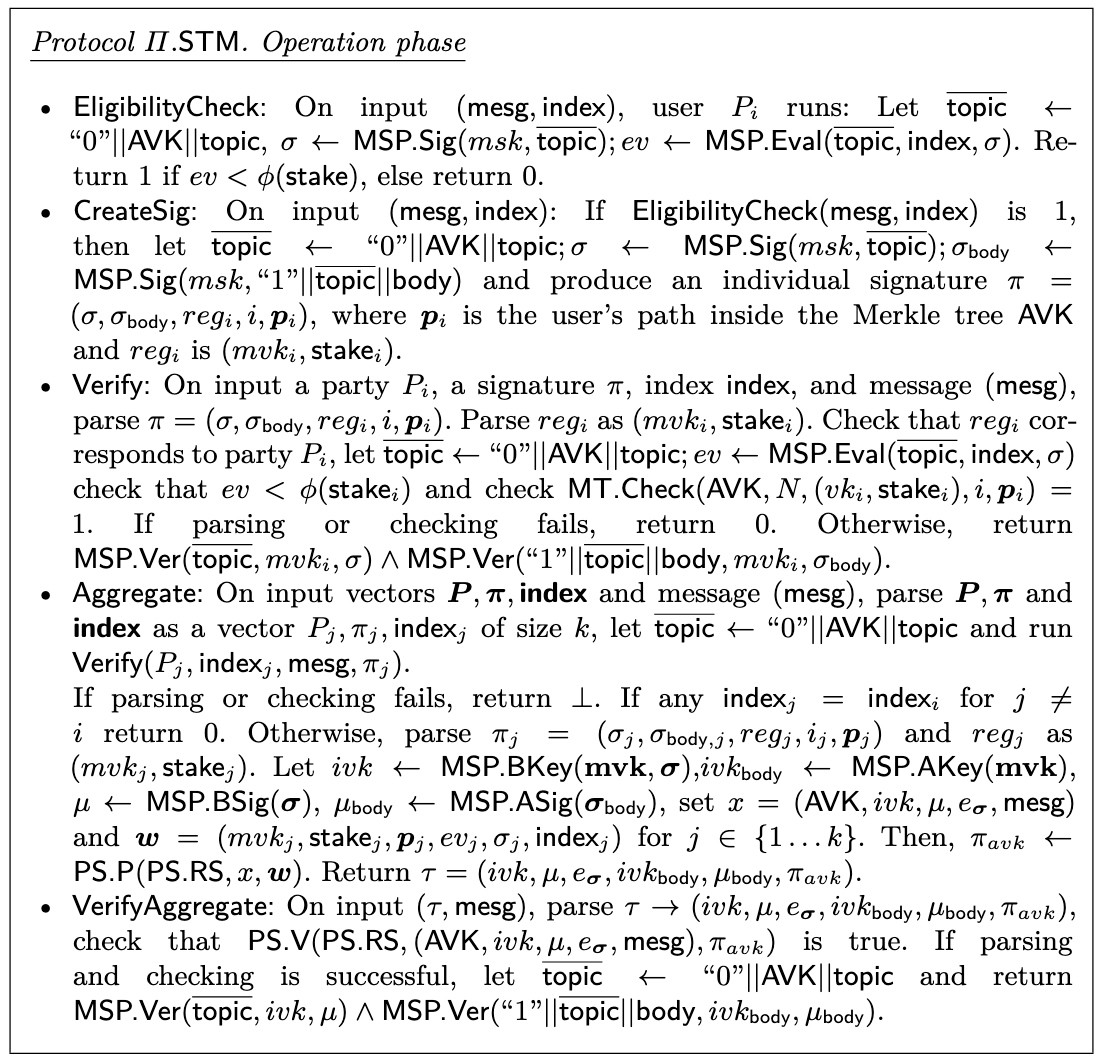
\includegraphics[width=1\linewidth]{1.png}

% \noindent\textbf{Notation.}
% Let $\mathsf{mesg}\equiv(\mathsf{topic},\mathsf{body})$.  Let $\mathsf{AVK}$ be the Merkle root of the stake registration tree with universe size $N$.  For party $P_i$ we write $\mathsf{reg}_i=(mvk_i,\mathsf{stake}_i)$ and $p_i$ for the Merkle path of $\mathsf{reg}_i$ at position $i$.  String concatenation is written ``$\Vert$''.  The MSP algorithms are as in the previous subsection.

% \begin{itemize}
%   \item \textbf{EligibilityCheck}: On input $(\mathsf{mesg},\mathsf{index})$, user $P_i$ runs:
%   \(
%     \mathsf{topic'} \leftarrow \text{``0''}\,\Vert\,\mathsf{AVK}\,\Vert\,\mathsf{topic},\qquad
%     \sigma \leftarrow \mathsf{MSP.Sig}(\mathsf{msk},\mathsf{topic'}),\qquad
%     ev \leftarrow \mathsf{MSP.Eval}(\mathsf{topic'},\mathsf{index},\sigma).
%   \)
%   Return $1$ if $ev<\phi(\mathsf{stake}_i)$, else return $0$.

%   \item \textbf{CreateSig}: On input $(\mathsf{mesg},\mathsf{index})$, if $\mathsf{EligibilityCheck}(\mathsf{mesg},\mathsf{index})=1$, then let
%   \(
%     \mathsf{topic'} \leftarrow \text{``0''}\,\Vert\,\mathsf{AVK}\,\Vert\,\mathsf{topic},\qquad
%     \sigma \leftarrow \mathsf{MSP.Sig}(\mathsf{msk},\mathsf{topic'}),\qquad
%     \sigma_{\mathsf{body}} \leftarrow \mathsf{MSP.Sig}(\mathsf{msk},\text{``1''}\,\Vert\,\mathsf{topic'}\,\Vert\,\mathsf{body}).
%   \)
%   Produce the individual signature
%   \(
%     \pi \;=\; (\sigma,\ \sigma_{\mathsf{body}},\ \mathsf{reg}_i,\ \iota_i,\ p_i),
%   \)
%   where $p_i$ is $P_i$'s Merkle path in the tree for $\mathsf{AVK}$ and $\mathsf{reg}_i=(mvk_i,\mathsf{stake}_i)$.

%   \item \textbf{Verify}: On input a party $P_i$, a signature $\pi$, an index $\mathsf{index}$, and a message $(\mathsf{mesg})$, parse
%   \(
%     \pi=(\sigma,\ \sigma_{\mathsf{body}},\ \mathsf{reg}_i,\ \iota_i,\ p_i),\quad
%     \mathsf{reg}_i=(mvk_i,\mathsf{stake}_i).
%   \)
%   Check that $\mathsf{reg}_i$ corresponds to party $P_i$.  Let
%   \(
%     \mathsf{topic'} \leftarrow \text{``0''}\,\Vert\,\mathsf{AVK}\,\Vert\,\mathsf{topic},\qquad
%     ev \leftarrow \mathsf{MSP.Eval}(\mathsf{topic'},\mathsf{index},\sigma).
%   \)
%   Check $ev<\phi(\mathsf{stake}_i)$ and
%   \(
%     \mathsf{MT.Check}(\mathsf{AVK},N,(mvk_i,\mathsf{stake}_i),i,p_i)=1.
%   \)
%   If any parsing or check fails, return $0$. Otherwise return
%   \(
%     \mathsf{MSP.Ver}(\mathsf{topic'},mvk_i,\sigma)\ \wedge\
%     \mathsf{MSP.Ver}(\text{``1''}\,\Vert\,\mathsf{topic'}\,\Vert\,\mathsf{body},mvk_i,\sigma_{\mathsf{body}}).
%   \)

%   \item \textbf{Aggregate}: On input vectors $\mathbf{P},\ \boldsymbol{\pi},\ \mathbf{index}$ and message $(\mathsf{mesg})$, parse
%   \(
%     \mathbf{P}=\{P_j\}_{j=1}^k,\quad \boldsymbol{\pi}=\{\pi_j\}_{j=1}^k,\quad \mathbf{index}=\{\mathsf{index}_j\}_{j=1}^k.
%   \)
%   Let $\mathsf{topic'}\leftarrow \text{``0''}\,\Vert\,\mathsf{AVK}\,\Vert\,\mathsf{topic}$ and run
%   \(
%     \mathsf{Verify}(P_j,\ \pi_j,\ \mathsf{index}_j,\ \mathsf{mesg})\quad\text{for all }j\in\{1,\dots,k\}.
%   \)
%   If parsing or any check fails, return $\bot$. If there exist $j\neq i$ with $\mathsf{index}_j=\mathsf{index}_i$, return $0$.
%   Otherwise, for each $j$ parse
%   \(
%     \pi_j=(\sigma_j,\ \sigma_{\mathsf{body},j},\ \mathsf{reg}_j,\ \iota_j,\ p_j),\quad
%     \mathsf{reg}_j=(mvk_j,\mathsf{stake}_j).
%   \)
%   Compute
%   \(
%     ivk \leftarrow \mathsf{MSP.BKey}(\mathbf{mvk},e_{\boldsymbol{\sigma}}),\qquad
%     ivk_{\mathsf{body}} \leftarrow \mathsf{MSP.AKey}(\mathbf{mvk}),
%   \)
%   \(
%     (\mu,e_{\boldsymbol{\sigma}}) \leftarrow \mathsf{MSP.BSig}(\boldsymbol{\sigma}),\qquad
%     \mu_{\mathsf{body}} \leftarrow \mathsf{MSP.ASig}(\boldsymbol{\sigma}_{\mathsf{body}}).
%   \)
%   Set the public statement and witness for the proof system $\mathsf{PS}$ as
%   \(
%     x \leftarrow (\mathsf{AVK},ivk,\mu,e_{\boldsymbol{\sigma}},\mathsf{mesg}),\qquad
%     w \leftarrow \{(mvk_j,\mathsf{stake}_j,p_j,ev_j,\sigma_j,\mathsf{index}_j)\}_{j=1}^k.
%   \)
%   Produce $\tau_{\mathsf{avk}} \leftarrow \mathsf{PS.P}(\mathsf{PS.RS},x,w)$ and output the aggregate
%   \(
%     \tau \;=\; (ivk,\ \mu,\ e_{\boldsymbol{\sigma}},\ ivk_{\mathsf{body}},\ \mu_{\mathsf{body}},\ \tau_{\mathsf{avk}}).
%   \)

%   \item \textbf{VerifyAggregate}: On input $(\tau,\mathsf{mesg})$, parse
%   \(
%     \tau \to (ivk,\ \mu,\ e_{\boldsymbol{\sigma}},\ ivk_{\mathsf{body}},\ \mu_{\mathsf{body}},\ \tau_{\mathsf{avk}}).
%   \)
%   Check that
%   \(
%     \mathsf{PS.V}(\mathsf{PS.RS},\ (\mathsf{AVK},ivk,\mu,e_{\boldsymbol{\sigma}},\mathsf{mesg}),\ \tau_{\mathsf{avk}})\ \text{ is true}.
%   \)
%   If parsing and checking succeed, let $\mathsf{topic'}\leftarrow \text{``0''}\,\Vert\,\mathsf{AVK}\,\Vert\,\mathsf{topic}$ and return
%   \(
%     \mathsf{MSP.Ver}(\mathsf{topic'},ivk,\mu)\ \wedge\
%     \mathsf{MSP.Ver}(\text{``1''}\,\Vert\,\mathsf{topic'}\,\Vert\,\mathsf{body},ivk_{\mathsf{body}},\mu_{\mathsf{body}}).
%   \)
% \end{itemize}



% \subsection{Relations for Mithril (latest version)}

% We state the relations we plan to prove in a SNARK. Compared to the paper's generic presentation, we inline the aggregated verification and range/uniqueness checks that the circuit already enforces.

% \paragraph{Public input (statement).}
% \(
%   x \ =\ \big(\mathsf{AVK},\ ivk,\ ivk_{\mathsf{body}},\ \mu,\ e_{\boldsymbol{\sigma}},\ \textsf{mesg}\big)\, .
% \)

% \paragraph{Witness.}
% \(
%   w \ =\ \big\{(mvk_i,\ \mathsf{stake}_i,\ p_i,\ ev_i,\ \sigma_i,\ \mathsf{index}_i)\big\}_{i=1}^k\, .
% \)

% \paragraph{Constraints.}
% \begin{enumerate}
%   \item \textbf{Aggregated keys and signature.}
%   \(
%     ivk \ =\ \mathsf{MSP.BKey}(\mathbf{mvk}, e_{\boldsymbol{\sigma}})\,,\qquad
%     ivk_{\mathsf{body}} \ =\ \mathsf{MSP.AKey}(\mathbf{mvk})\,,\qquad
%     (\mu,e_{\boldsymbol{\sigma}}) \ =\ \mathsf{MSP.BSig}(\boldsymbol{\sigma})\, .
%   \)
%   with $e_{\boldsymbol{\sigma}}=H_p(\boldsymbol{\sigma})$ and $e_i=H_{\lambda}(i,e_{\boldsymbol{\sigma}})$. % :contentReference[oaicite:9]{index=9} % :contentReference[oaicite:10]{index=10} % :contentReference[oaicite:11]{index=11}
%   \item \textbf{Membership in the AVK Merkle tree.} For each $i\in\{1,\ldots,k\}$, the pair $(mvk_i,\mathsf{stake}_i)$ opens along path $p_i$ to the Merkle root $\mathsf{AVK}$ over a universe of $N$ registered keys. % :contentReference[oaicite:12]{index=12}
%   \item \textbf{Index bounds and uniqueness.} For all $i$, $0\le \mathsf{index}_i \le m$, and for $i\ne j$, $\mathsf{index}_i \ne \mathsf{index}_j$. (Enforced via range checks and collision checks in-circuit.) % :contentReference[oaicite:13]{index=13}
%   \item \textbf{Eligibility values.} For each $i$, compute
%   \(
%     ev_i \ =\ \mathsf{MSP.Eval}(\textsf{topic},\mathsf{index}_i,\sigma_i)\, ,
%   \)
%   using the dense mapping associated to the chosen instantiation (RO-based or Elligator-Squared-based). % :contentReference[oaicite:14]{index=14} % :contentReference[oaicite:15]{index=15}
%   \item \textbf{Stake threshold per lottery.} For each $i$, enforce $ev_i \le \phi(\mathsf{stake}_i)$ for the scaling function $\phi(\cdot)$. % :contentReference[oaicite:16]{index=16}
%   \item \textbf{Aggregated verification inside the circuit.} The circuit implements $\mathsf{MSP.Ver}(\textsf{msghash}, ivk,\mu)=1$, which (by the batching lemma) is equivalent to all underlying $\mathsf{MSP.Ver}(\textsf{msghash},mvk_i,\sigma_i)$ passing, except with negligible probability over the random-oracle coins that derive $(e_{\boldsymbol{\sigma}},\{e_i\})$. % :contentReference[oaicite:17]{index=17} % :contentReference[oaicite:18]{index=18}
% \end{enumerate}

% \paragraph{Notes.}
% \begin{itemize}
%   \item The use of $H_p$ for $e_{\boldsymbol{\sigma}}$ and $H_{\lambda}$ for short exponents follows the paper's batching construction and keeps hash oracles \emph{out of} the arithmetic circuit when desired. % :contentReference[oaicite:19]{index=19} % :contentReference[oaicite:20]{index=20}
%   \item Either the RO-based mapping $M^{\mathrm{R}}_{\textsf{msg},\textsf{index}}$ or the Elligator-Squared mapping $M^{\mathrm{E}}_{\textsf{msg},\textsf{index}}$ can be plugged in; the latter avoids hashing witness elements (the signatures) directly inside the circuit. % :contentReference[oaicite:21]{index=21} % :contentReference[oaicite:22]{index=22}
% \end{itemize}


\subsection{Relation for Mithril}

The proof system is defined over the language $\mathcal{L}_{\mathsf{avk}}$, which describes statements $x$ that admit a witness $w$ such that $R_{\mathsf{avk}}(x,w)=1$. Concretely, statements and witnesses are
\[
  x \;=\; (\mathsf{AVK},\, ivk,\, ivk_{\mathsf{body}},\, \mu,\, e_{\boldsymbol{\sigma}},\, \mathsf{mesg}) ,
  \qquad
  w \;=\; \big\{(mvk_i,\, \mathsf{stake}_i,\, p_i,\, ev_i,\, \sigma_i,\, \mathsf{index}_i)\big\}_{i=1}^{k}.
\]
The relation $R_{\mathsf{avk}}$ is parameterized by public values $(N, m, k, \phi)$.

\medskip
\noindent $R_{\mathsf{avk}}(x,w)=1$ if and only if all of the following hold:
\begin{itemize}
  \item $ivk=\mathsf{MSP.BKey}(\mathbf{mvk},\, e_{\boldsymbol{\sigma}})$ and $ivk_{\mathsf{body}}=\mathsf{MSP.AKey}(\mathbf{mvk})$, where $\mathbf{mvk}=(mvk_1,\ldots,mvk_k)$.
  \item $(\mu,\, e_{\boldsymbol{\sigma}})=\mathsf{MSP.BSig}(\boldsymbol{\sigma})$, where $\boldsymbol{\sigma}=(\sigma_1,\ldots,\sigma_k)$.
  \item For all $i$: $\mathsf{index}_i \le m$, and for all $i\neq j$: $\mathsf{index}_i \neq \mathsf{index}_j$.
  \item For each $i\in\{1,\ldots,k\}$: the pair $(mvk_i,\mathsf{stake}_i)$ lies in the Merkle tree with root $\mathsf{AVK}$ and universe size $N$, following path $p_i$.
  \item For each $i\in\{1,\ldots,k\}$: $\mathsf{MSP.Eval}(\mathsf{topic},\, \mathsf{index}_i,\, \sigma_i)=ev_i$.
  \item For each $i\in\{1,\ldots,k\}$: $ev_i \le \phi(\mathsf{stake}_i)$.
\end{itemize}

\subsection{Why Snarkify Mithril —— ZK Cross-Chain Bridge}

\begin{figure}[htbp]
  \centering
  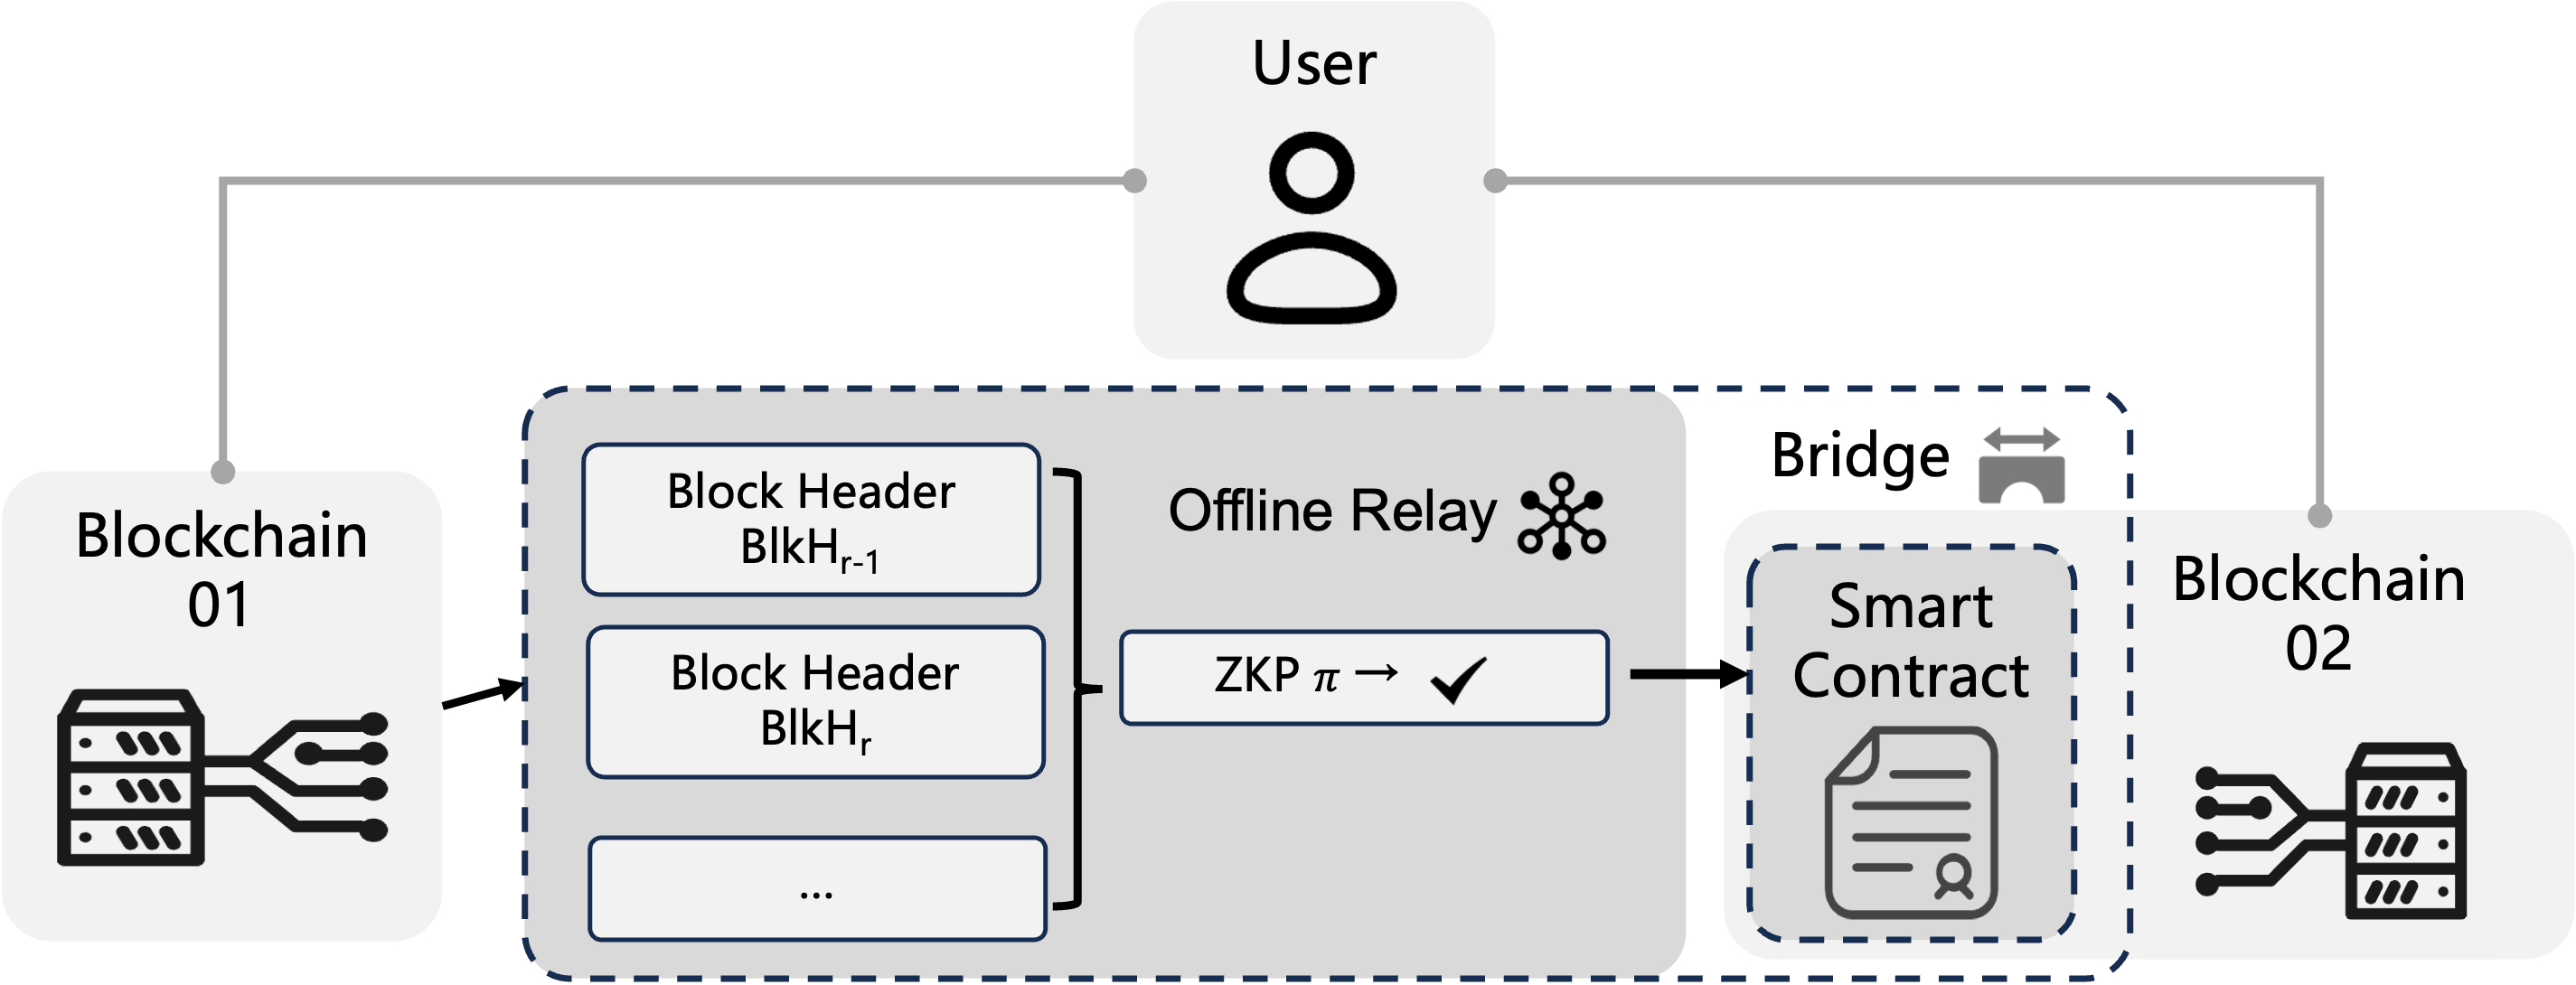
\includegraphics[width=0.88\linewidth]{2.png}
%   \caption{Off-chain relay produces a succinct ZKP $\pi$ for a Mithril-certified statement; the on-chain verifier on \emph{Blockchain 02} checks $\pi$ and enforces application logic.}
  \label{fig:bridge-architecture}
\end{figure}

We SNARKify Mithril to build practical cross-chain bridges: the aggregator proves off-chain that a Mithril certificate is valid (weighted BLS aggregations, eligibility, index and Merkle checks), and the destination chain verifies only a succinct proof. This shifts heavy pairing/MSM/hash work off-chain, makes on-chain cost small and stable (single verifier call), removes the need for native BLS support, and preserves Mithril’s stake-weighted security guarantees under an untrusted relay.

% \paragraph{Motivation.}
% A raw Mithril certificate bundles (i) BLS-based aggregated verification for the \emph{topic} and \emph{body}, (ii) derivation of the seed $e_{\boldsymbol{\sigma}}$ and short exponents $e_i$, (iii) a weighted MSM over keys and signatures, (iv) per-signer eligibility via $\mathsf{MSP.Eval}$, (v) index range \& uniqueness checks, and (vi) Merkle membership of $(mvk_i,\mathsf{stake}_i)$ in the registration root $\mathsf{AVK}$. Executing these checks directly on a destination chain is expensive and, on many platforms, even \emph{infeasible} (e.g., missing native BLS12-381 support or high gas for large MSMs and $O(n^2)$ uniqueness checks). To build a practical, self-verifying \emph{bridge}, we therefore \emph{SNARKify} Mithril: heavy computation happens off-chain, while the chain verifies a small proof.

% \paragraph{Design objective.}
% Compress the following relation into a single succinct proof:
% \[
%   R_{\mathsf{bridge}}(x,w)\ \equiv\ \Big(
%     R_{\mathsf{avk}}(x,w)
%     \ \wedge\
%     \mathsf{MSP.Ver}(\text{``0''}\Vert\mathsf{AVK}\Vert\mathsf{topic},\, ivk,\, \mu)
%     \ \wedge\
%     \mathsf{MSP.Ver}(\text{``1''}\Vert\mathsf{AVK}\Vert\mathsf{topic}\Vert\mathsf{body},\, ivk_{\mathsf{body}},\, \mu_{\mathsf{body}})
%   \Big),
% \]
% where $x=(\mathsf{AVK}, ivk, ivk_{\mathsf{body}}, \mu, \mu_{\mathsf{body}}, e_{\boldsymbol{\sigma}}, \mathsf{mesg})$ and $w$ contains the per-signer witnesses (keys, stakes, paths, indices, signatures, and eligibility values). The off-chain relay proves $R_{\mathsf{bridge}}(x,w)=1$ and submits only the succinct proof $\pi$ and the public inputs $x$ on-chain.

% \paragraph{Security and trust model.}
% The relay/aggregator is \emph{untrusted}: correctness follows from SNARK knowledge soundness, Merkle binding, collision resistance of the hashes used for $e_{\boldsymbol{\sigma}}$ and $e_i$, and BLS unforgeability. If $\pi$ verifies on-chain, then (1) a stake-weighted threshold of eligible signers attested the message, (2) all signers are registered under $\mathsf{AVK}$, (3) indices are valid and unique, and (4) both aggregated BLS equations hold—exactly mirroring the native Mithril checks.

% \paragraph{Practical benefits for bridges.}
% \begin{itemize}
%   \item \textbf{Constant/low on-chain cost.} On-chain work reduces to a single SNARK verification (plus cheap public-input checks), independent of the number of signers $k$.
%   \item \textbf{Portability across chains.} The destination chain only needs a verifier for the chosen proof system (e.g., Groth16/PLONK/Halo2 via appropriate precompiles), not native BLS verifiers or large MSM support.
%   \item \textbf{Latency and UX.} Off-chain proving amortizes heavy cryptography; users receive fast, one-shot on-chain verification and finality for cross-chain actions.
%   \item \textbf{Security preservation.} The proof attests the \emph{same} semantics as Mithril’s operation phase, preserving stake-weighted guarantees without trusting the relay.
% \end{itemize}

% \paragraph{Workflow.}
% (1) The relay collects source-chain artifacts (e.g., headers or checkpoints) and a Mithril certificate; (2) it proves $R_{\mathsf{bridge}}$ off-chain to obtain $\pi$; (3) a smart contract on the destination chain verifies $\pi$ and, if valid, executes the bridge logic tied to $(\mathsf{topic},\mathsf{body})$ (Fig.~\ref{fig:bridge-architecture}). This \emph{SNARKified} pipeline enables practical, secure, and chain-agnostic Mithril-based bridges.



% \section{Snarkifying Mithril(Practical)}

\section{Snarkifying Mithril (Practical)}
\label{sec:snarkifying-mithril-practical}

This section implements a Halo2-based zero-knowledge cross-chain protocol instantiated with Mithril. The circuit covers: (i) unweighted BLS multisignature aggregation ($\mathsf{MSP.A}$), (ii) seed-weighted BLS aggregation ($\mathsf{MSP.B}$), (iii) lottery index range \& uniqueness checks, (iv) eligibility/threshold checks against stake, and (v) Merkle membership checks for registered signers. The experimental environment matches the previous section.

\subsection{Experimental Tasks}
\begin{itemize}
  \item \textbf{MSP.A (baseline aggregation).} Implements the straightforward BLS aggregation and in-circuit pairing check $e(\mu,g_2)=e(H_{\mathbb{G}_1}(\text{``M''}\Vert msg), ivk)$. We measure proving time, proof size, and verification time as the number of aggregated signatures grows.
  \item \textbf{MSP.B (seed-weighted aggregation).} Extends aggregation with per-signer short exponents $e_i \leftarrow H_\lambda(i,e_{\boldsymbol{\sigma}})$ and $(\mu,e_{\boldsymbol{\sigma}})$ where $e_{\boldsymbol{\sigma}}\leftarrow H_p(\boldsymbol{\sigma})$. The circuit proves the weighted pairing equation. We observe higher proving cost due to hashing and multi-scalar multiplications (MSMs) with weights.
  \item \textbf{Lottery index check.} Ensures $\mathsf{index}_i\!\le m$ for all $i$ and $\mathsf{index}_i\!\ne\!\mathsf{index}_j$ for $i\ne j$. The uniqueness constraint induces $O(n^2)$ comparisons; we report scaling behavior.
  \item \textbf{Eligibility/threshold check.} For each signer, enforces $ev_i=\mathsf{MSP.Eval}(\mathsf{topic},\mathsf{index}_i,\sigma_i)$ and $ev_i \le \phi(\mathsf{stake}_i)$. The circuit cost grows roughly linearly in the number of checked signers.
\end{itemize}

\subsection{Benchmark Tables}

\begin{table}[htbp]
  \centering
  \caption{MSP.A (unweighted aggregation) results}
  \renewcommand{\arraystretch}{0.9}
  \setlength{\tabcolsep}{10pt}
  \begin{tabular}{lcccccc}
    \toprule
    \textbf{aggregated signatures} & \textbf{2} & \textbf{200} & \textbf{2000} & \textbf{4000} & \textbf{6000} & \textbf{8000} \\
    \midrule
    Proving time (s)     & 19.17 & 29.51 & 72.89 & 123.67 & 181.38 & 226.84 \\
    Proof size (bytes)   & 3072  & 4128  & 11424 & 18944  & 26944  & 34944  \\
    Verification time (ms) & 20.93 & 9.09  & 19.95 & 16.03  & 20.25  & 55.16  \\
    \bottomrule
  \end{tabular}
  \label{tab:mspa_benchmark_en}
\end{table}


\begin{table}[htbp]
  \centering
  \caption{MSP.B (seed-weighted aggregation) results}
  \renewcommand{\arraystretch}{0.9}
  \setlength{\tabcolsep}{10pt}
  \begin{tabular}{lcccccc}
    \toprule
    \textbf{aggregated signatures} & \textbf{8} & \textbf{16} & \textbf{32} & \textbf{64} & \textbf{128} & \textbf{256} \\
    \midrule
    Proving time (s)     & 35.73 & 48.48 & 65.37 & 103.75 & 184.02 & 327.30 \\
    Proof size (bytes)   & 5856  & 7936  & 10944 & 17312  & 30240  & 55744  \\
    Verification time (ms) & 10.30 & 14.68 & 15.05 & 14.54 & 24.51  & 69.35  \\
    \bottomrule
  \end{tabular}
  \label{tab:mspb_benchmark_en}
\end{table}


\begin{table}[htbp]
  \centering
  \caption{Lottery index check results (range \& uniqueness)}
  \renewcommand{\arraystretch}{0.9}
  \setlength{\tabcolsep}{10pt}
  \begin{tabular}{lccccc}
    \toprule
    \textbf{indices} & \textbf{128} & \textbf{256} & \textbf{512} & \textbf{1024} & \textbf{2048} \\
    \midrule
    Proving time (s)     & 4.08 & 6.77  & 13.41 & 37.39 & 122.49 \\
    Proof size (bytes)   & 960  & 1920  & 4576  & 14944 & 14944 \\
    Verification time (ms) & 5.05 & 6.15 & 9.42  & 15.10 & 13.08 \\
    \bottomrule
  \end{tabular}
  \label{tab:index_check_benchmark_en}
\end{table}


\begin{table}[htbp]
  \centering
  \caption{Eligibility / stake-threshold check results}
  \renewcommand{\arraystretch}{0.9}
  \setlength{\tabcolsep}{10pt}
  \begin{tabular}{lccccc}
    \toprule
    \textbf{checks} & \textbf{128} & \textbf{256} & \textbf{512} & \textbf{1024} & \textbf{2048} \\
    \midrule
    Proving time (s)     & 10.14 & 12.78 & 17.36 & 26.39 & 44.56 \\
    Proof size (bytes)   & 1344  & 1920  & 2848  & 4800  & 8832 \\
    Verification time (ms) & 6.77  & 6.39  & 7.10  & 11.24 & 12.59 \\
    \bottomrule
  \end{tabular}
  \label{tab:eligibility_check_benchmark_en}
\end{table}


\begin{table}[htbp]
\centering
\caption{Merkle membership proof results (transposed, with stake)}
\renewcommand{\arraystretch}{0.9}
\setlength{\tabcolsep}{8pt}
\begin{tabular}{lccccccc}
\toprule
 & \textbf{16} & \textbf{32} & \textbf{64} & \textbf{128} & \textbf{256} & \textbf{512} & \textbf{1024} \\
\midrule
original proofs    & 32    & 64    & 128   & 256   & 512   & 1024  & 2048   \\
Proving time (s)     & 5.68  & 7.60  & 13.44 & 23.29 & 48.63 & 100.05 & 213.25 \\
Proof size (bytes)    & 704     & 1056    & 2112    & 3872    & 8448    & 17600    & 38016    \\
Verification time (ms) & 6.57  & 4.47  & 7.64  & 8.13  & 11.65 & 13.61  & 20.31  \\
\bottomrule
\end{tabular}
\label{tab:merkle_proof_benchmark_transposed}
\end{table}




\newpage

\section{Snarkifying Mithril(Theoretical)}



\subsection{SNARK}
A SNARK for a relation $\mathcal{R}$ is a triple of PPT algorithms $\Pi = (\mathsf{Setup}, \mathsf{Prove}, \mathsf{Verify})$ defined as follows:


\begin{itemize}
    \item $  \mathsf{srs} \leftarrow \mathsf{Setup}(1^\lambda)$:On input security parameter $\lambda$
, it outputs a structured reference string $\mathsf{srs}$.   
    \item $\pi \leftarrow \mathsf{Prove}(\mathsf{srs}, x, w)$: On input $\mathsf{srs}$, a statement $x$ and a witness $w$ such that $(x, w) \in \mathcal{R}$, output a proof $\pi$.
    \item $0/1 \leftarrow\mathsf{Verify}(\mathsf{srs},x,\pi) $:On input $\mathsf{srs}$, a statement $x$, and a
proof $\pi$, it outputs either 1 indicating accepting the statement or 0 for rejecting it.
\end{itemize}

\subsection{BLS}
$\Pi_{BLS} = (Setup,Sign,Ver)$
\begin{itemize}
    \item $(sk,vk = g_1^{sk}) \leftarrow Setup() $
    \item $\sigma \leftarrow Sign(sk,msg), \text{where  }\sigma = H(msg)^{sk}$
    \item $1/0 \leftarrow Ver(vk,\sigma,msg)$, check $e(g_1, \sigma) = e(\mathsf{vk}, H(msg))$
\end{itemize}

\subsection{Merkle tree}

$\Pi_{MT} = (Create,Check)$

\begin{itemize}
    \item $avk \leftarrow Create(\mathbf{VK})$
    \item $1/0 \leftarrow Check(vk,avk,path)$
\end{itemize}

\subsection{SNARK-based Mithril}


\[
\Pi_{\mathsf{F-Mithril}}
= (\mathsf{Register},
   \mathsf{EligibilityCheck}, \mathsf{CreateSig}, \mathsf{Verify},
   \mathsf{Aggregate}, \mathsf{VerifyAggregate})
\]

\[
\Pi_{\mathsf{SNARK-Mithril}}
= (\mathsf{PGen}, \mathsf{KGen}, \mathsf{Avk},
   \mathsf{AvkProve},
   \mathsf{AvkCheck}, \mathsf{Sig}, \mathsf{Ver},
   \mathsf{ASig}, \mathsf{AVer})
\]

\paragraph{Mithril.PGen()}
\begin{align*}
&srs \leftarrow \text{Setup}(1^\lambda)\\
&\text{return } srs 
\end{align*}

\paragraph{Mithril.KGen(pp)}
\begin{align*}
&sk \leftarrow \mathbb{Z}_q \\
&vk \leftarrow g_1^{sk} \\
&\text{return } (sk, vk)
\end{align*}

\paragraph{Mithril.Avk(\textbf{VK}, \textbf{w})}
\begin{align*}
&\textbf{WVK} \leftarrow \{(w_i, vk_i) : i \in [n]\} \\
&w \leftarrow \sum_{i \in [n]} w_i\\
&avk \leftarrow MT.\mathrm{Create}(\textbf{WVK}) \\
&\text{return } (avk,w)
\end{align*}

\paragraph{Mithril.AvkProve(VK, w, avk, path， srs)}
\begin{align*}
&\pi_1 \leftarrow \mathsf{SNARK.Prove}(srs, x = avk, w = (\textbf{VK}, \textbf{w}, \textbf{path})) \\
&\quad (\mathcal{R} = \{(x = avk, w = (\textbf{VK}, \textbf{w}, \textbf{path}))\quad |\\ & \quad \ \ \forall i \in [m],\ MT.\mathrm{Check}(avk, (w_i, vk_i), path_i) = 1 \}) \\
&\text{return } \pi_1
\end{align*}

\paragraph{Mithril.AvkCheck(avk, srs)}

\begin{align*}
&\text{return } \mathsf{SNARK.Verify}(srs, x = avk,\pi_1)
\end{align*}

\paragraph{Mithril.Sig(\text{sk, j, msg, w, w_{i})}}
\begin{align*}
% &\sigma \leftarrow \mathrm{BLS.Sign}(sk, (j|| msg|| w|| w_{i})) \\
&\sigma \leftarrow \mathrm{BLS.Sign}(sk, msg) \\
&\text{return } \sigma
\end{align*}

\paragraph{Mithril.Ver(vk, j, msg, \sigma, w, w_i)}
\begin{align*}
% &\text{if } MT.\mathrm{Check}(avk, N, (w_i, vk), j^*, \text{path}) \neq 1,\ \text{return } 0 \\
% &\text{return } \mathrm{BLS.Ver}(vk,\sigma, (j|| msg|| w|| w_{i})) 
&\text{return } \mathrm{BLS.Ver}(vk,\sigma, msg) 
\end{align*}

\paragraph{Mithril.ASig( S=$\{(\sigma_j,j) | j\  \in\  [m]\}$)}
\begin{align*}
&\boldsymbol{\sigma} \leftarrow [\{\sigma_j | j\  \in\  [m]\}] \\
&e_{\sigma} \leftarrow H_p(\boldsymbol{\sigma}) \\
&e_j \leftarrow H_\lambda(j, e_{\sigma}) \\
&\mu \leftarrow \prod_j \sigma_j^{e_j} \\
&\pi_2 \leftarrow SNARK.Prove(srs,x=(\mu, e_{\sigma}),w=(\boldsymbol{\sigma})) \\
&\quad (R = \{x=(\mu, e_{\sigma},,w),w=(\boldsymbol{\sigma})\quad|\quad \\
&\quad \ \ e_{\sigma} = H_p(\boldsymbol{\sigma}) \land e_j = H_\lambda(j, e_{\sigma}) \land \mu = \prod_j \sigma_j^{e_j} \})\\ 
% &\quad \ \ \land BLS.Ver(avk,\mu,ivk)\}\\
&\sigma^* \leftarrow (\mu, e_{\sigma},\pi_2) \\
&\text{return } \sigma^* 
\end{align*}

\paragraph{Mithril.AVer(ivk, msg, \sigma*, w)}
\begin{align*}
&r_1 \leftarrow \mathsf{SNARK.Verify}(srs, x = (\mu, e_{\sigma}),\pi_2)\\
&r_2 \leftarrow \mathsf{BLS.Ver}(ivk,\mu,msg) \\
&\textbf{return}\quad r_1 \land r_2
\end{align*}

(Here, ivk = $\prod_j vk_j^{e_j}$)


\subsection{Remained Questions}
\begin{enumerate}
    \item It is unclear how to incorporate weights into BLS signatures, especially when performing aggregation in BLS multisignatures.

In the case where all signers agree on the same message $m$, 
the aggregated signature can be written as
\[
\sigma_{agg} = \prod_{i} \sigma_i = H(m)^{\sum_i sk_i},
\]
and thus the corresponding aggregated public key is simply
\[
vk_{agg} = \prod_{i} vk_i.
\]
Verification then reduces to a single pairing equation
\[
e(g, \sigma_{agg}) \overset{?}{=} e(vk_{agg}, H(m)),
\]
which is compact and efficient.

However, when each signer signs a \emph{different} message $m_i$, 
the aggregated signature becomes
\[
\sigma_{agg} = \prod_{i} H(m_i)^{sk_i},
\]
for which there does not exist a single aggregated public key. 
Instead, the verification requires
\[
e(g, \sigma_{agg}) \overset{?}{=} \prod_{i} e(vk_i, H(m_i)),
\]
where every individual public key $vk_i$ and message $m_i$ 
must be explicitly included in the verification. 
This implies that, unlike the single-message case, 
the verification cost is not succinct, 
and the aggregation does not yield a compact verification procedure.

\item The smart contract needs to verify both the $\mathsf{Mithril.AvkCheck}$ and $\mathsf{Mithril.AVer}$ proofs, i.e., it must verify two SNARK proofs and one BLS signature.
\end{enumerate}


\section{Other Explorations}
We designed an optimization for workloads that require opening a large number of Merkle proofs.  Due to scenario-specific constraints, this approach may not be directly applicable to our current use case.\\


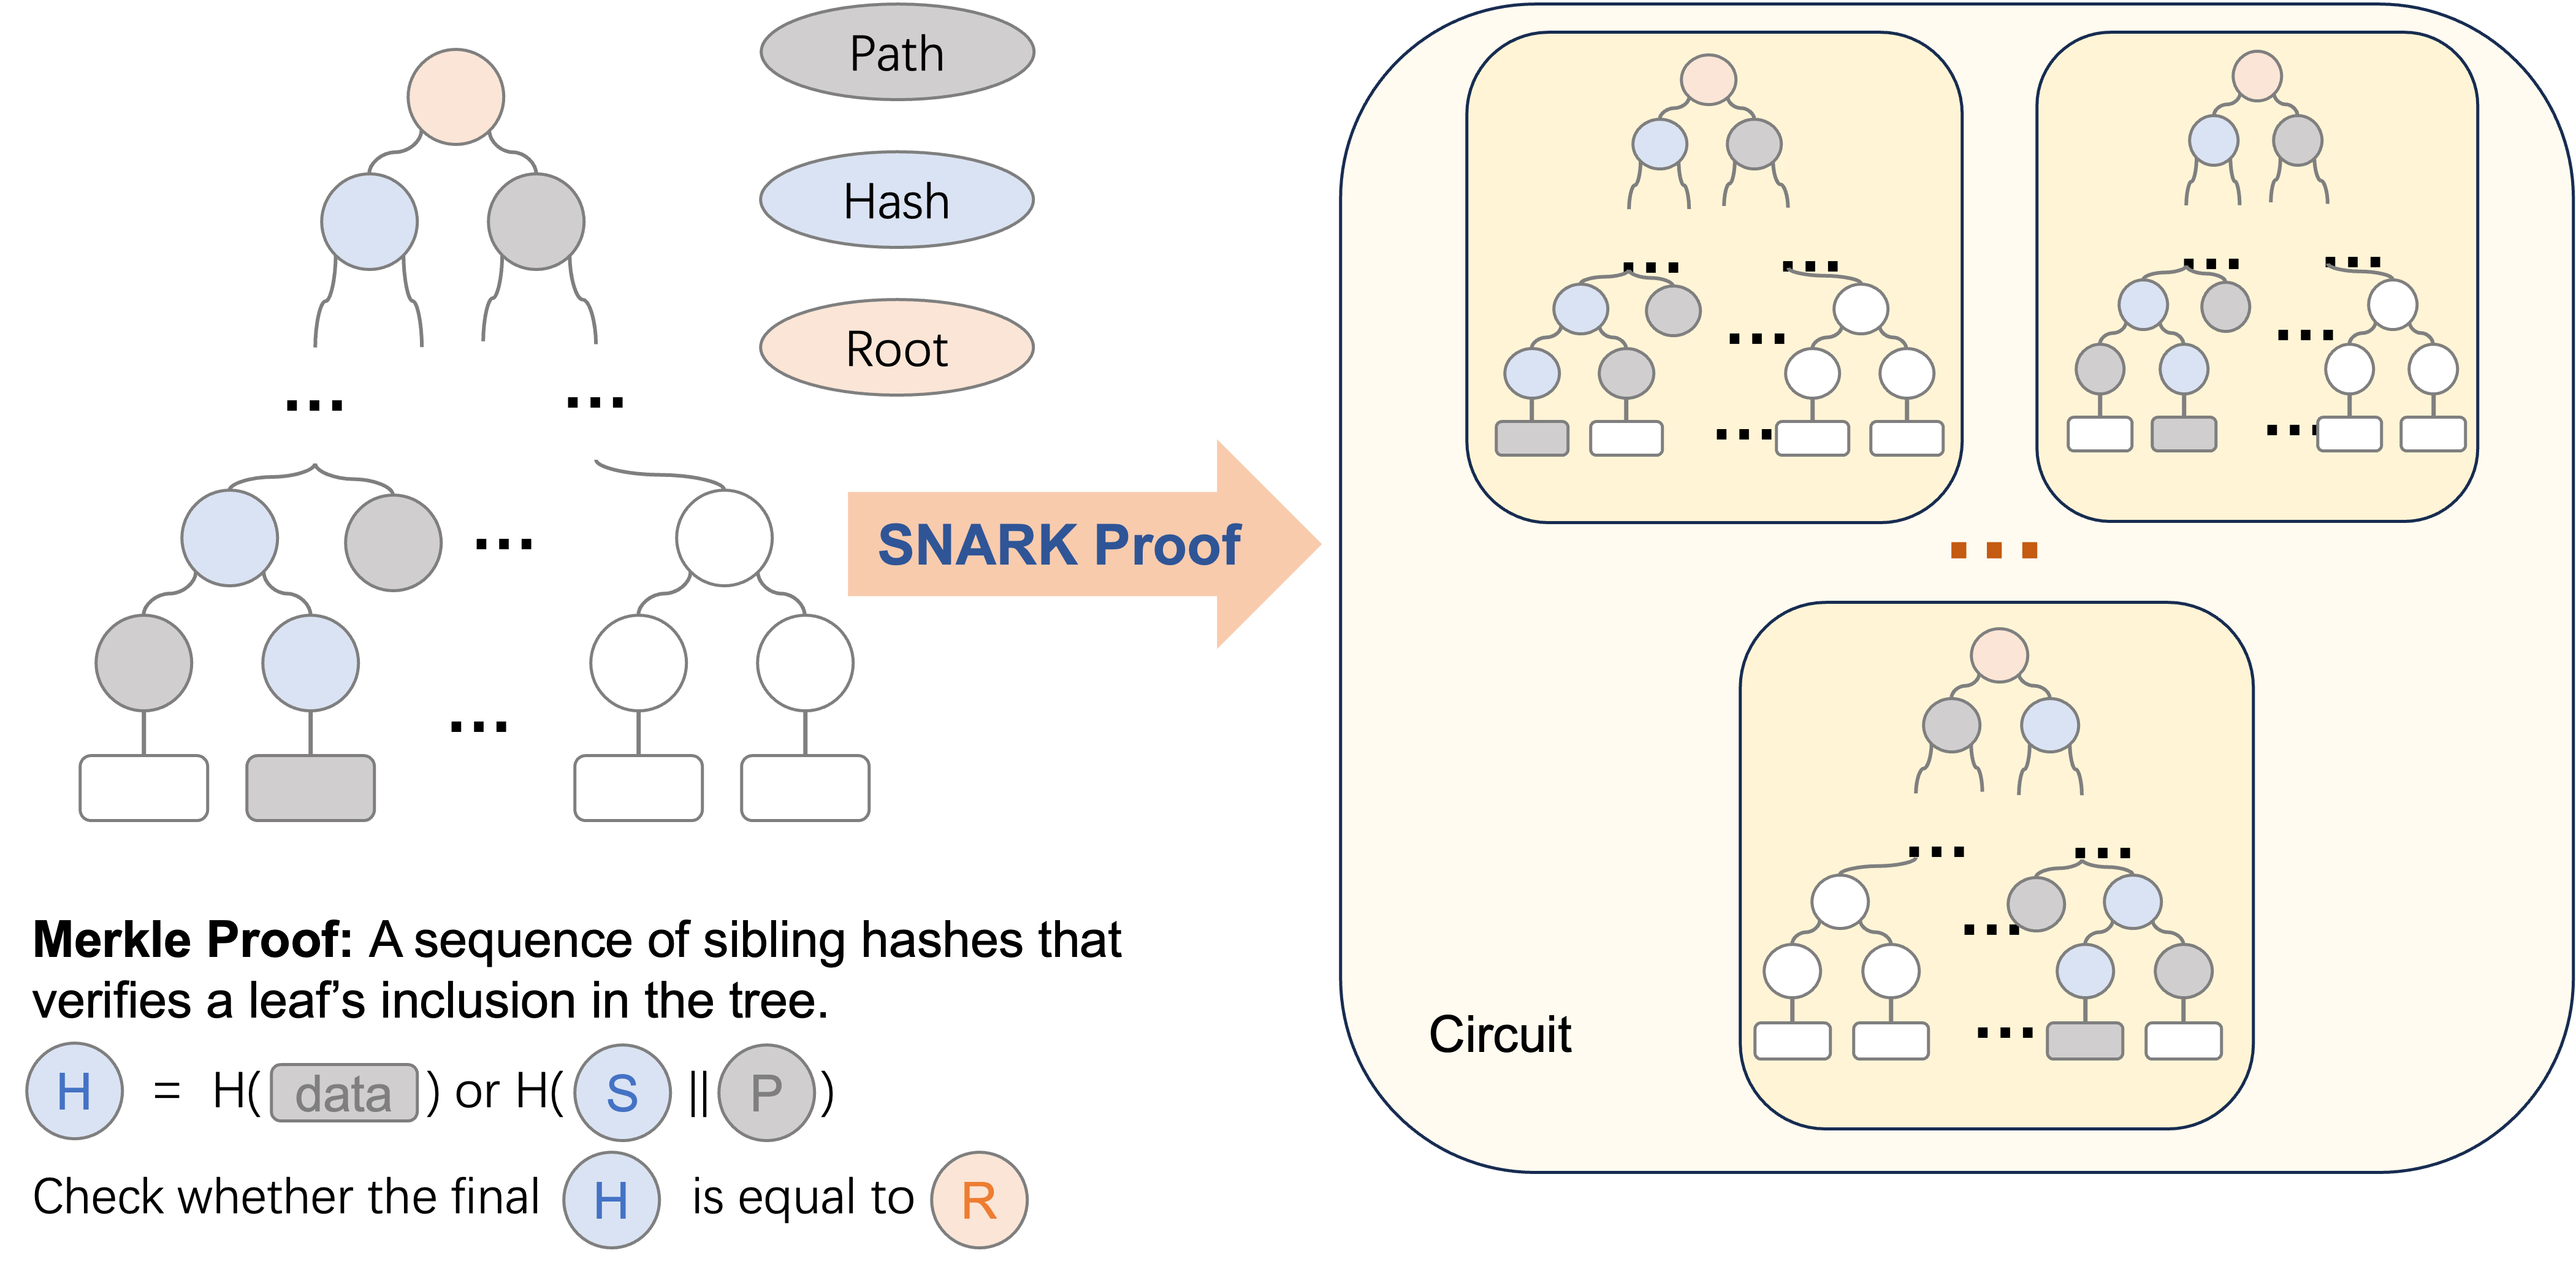
\includegraphics[width=1\linewidth]{33.png}\\

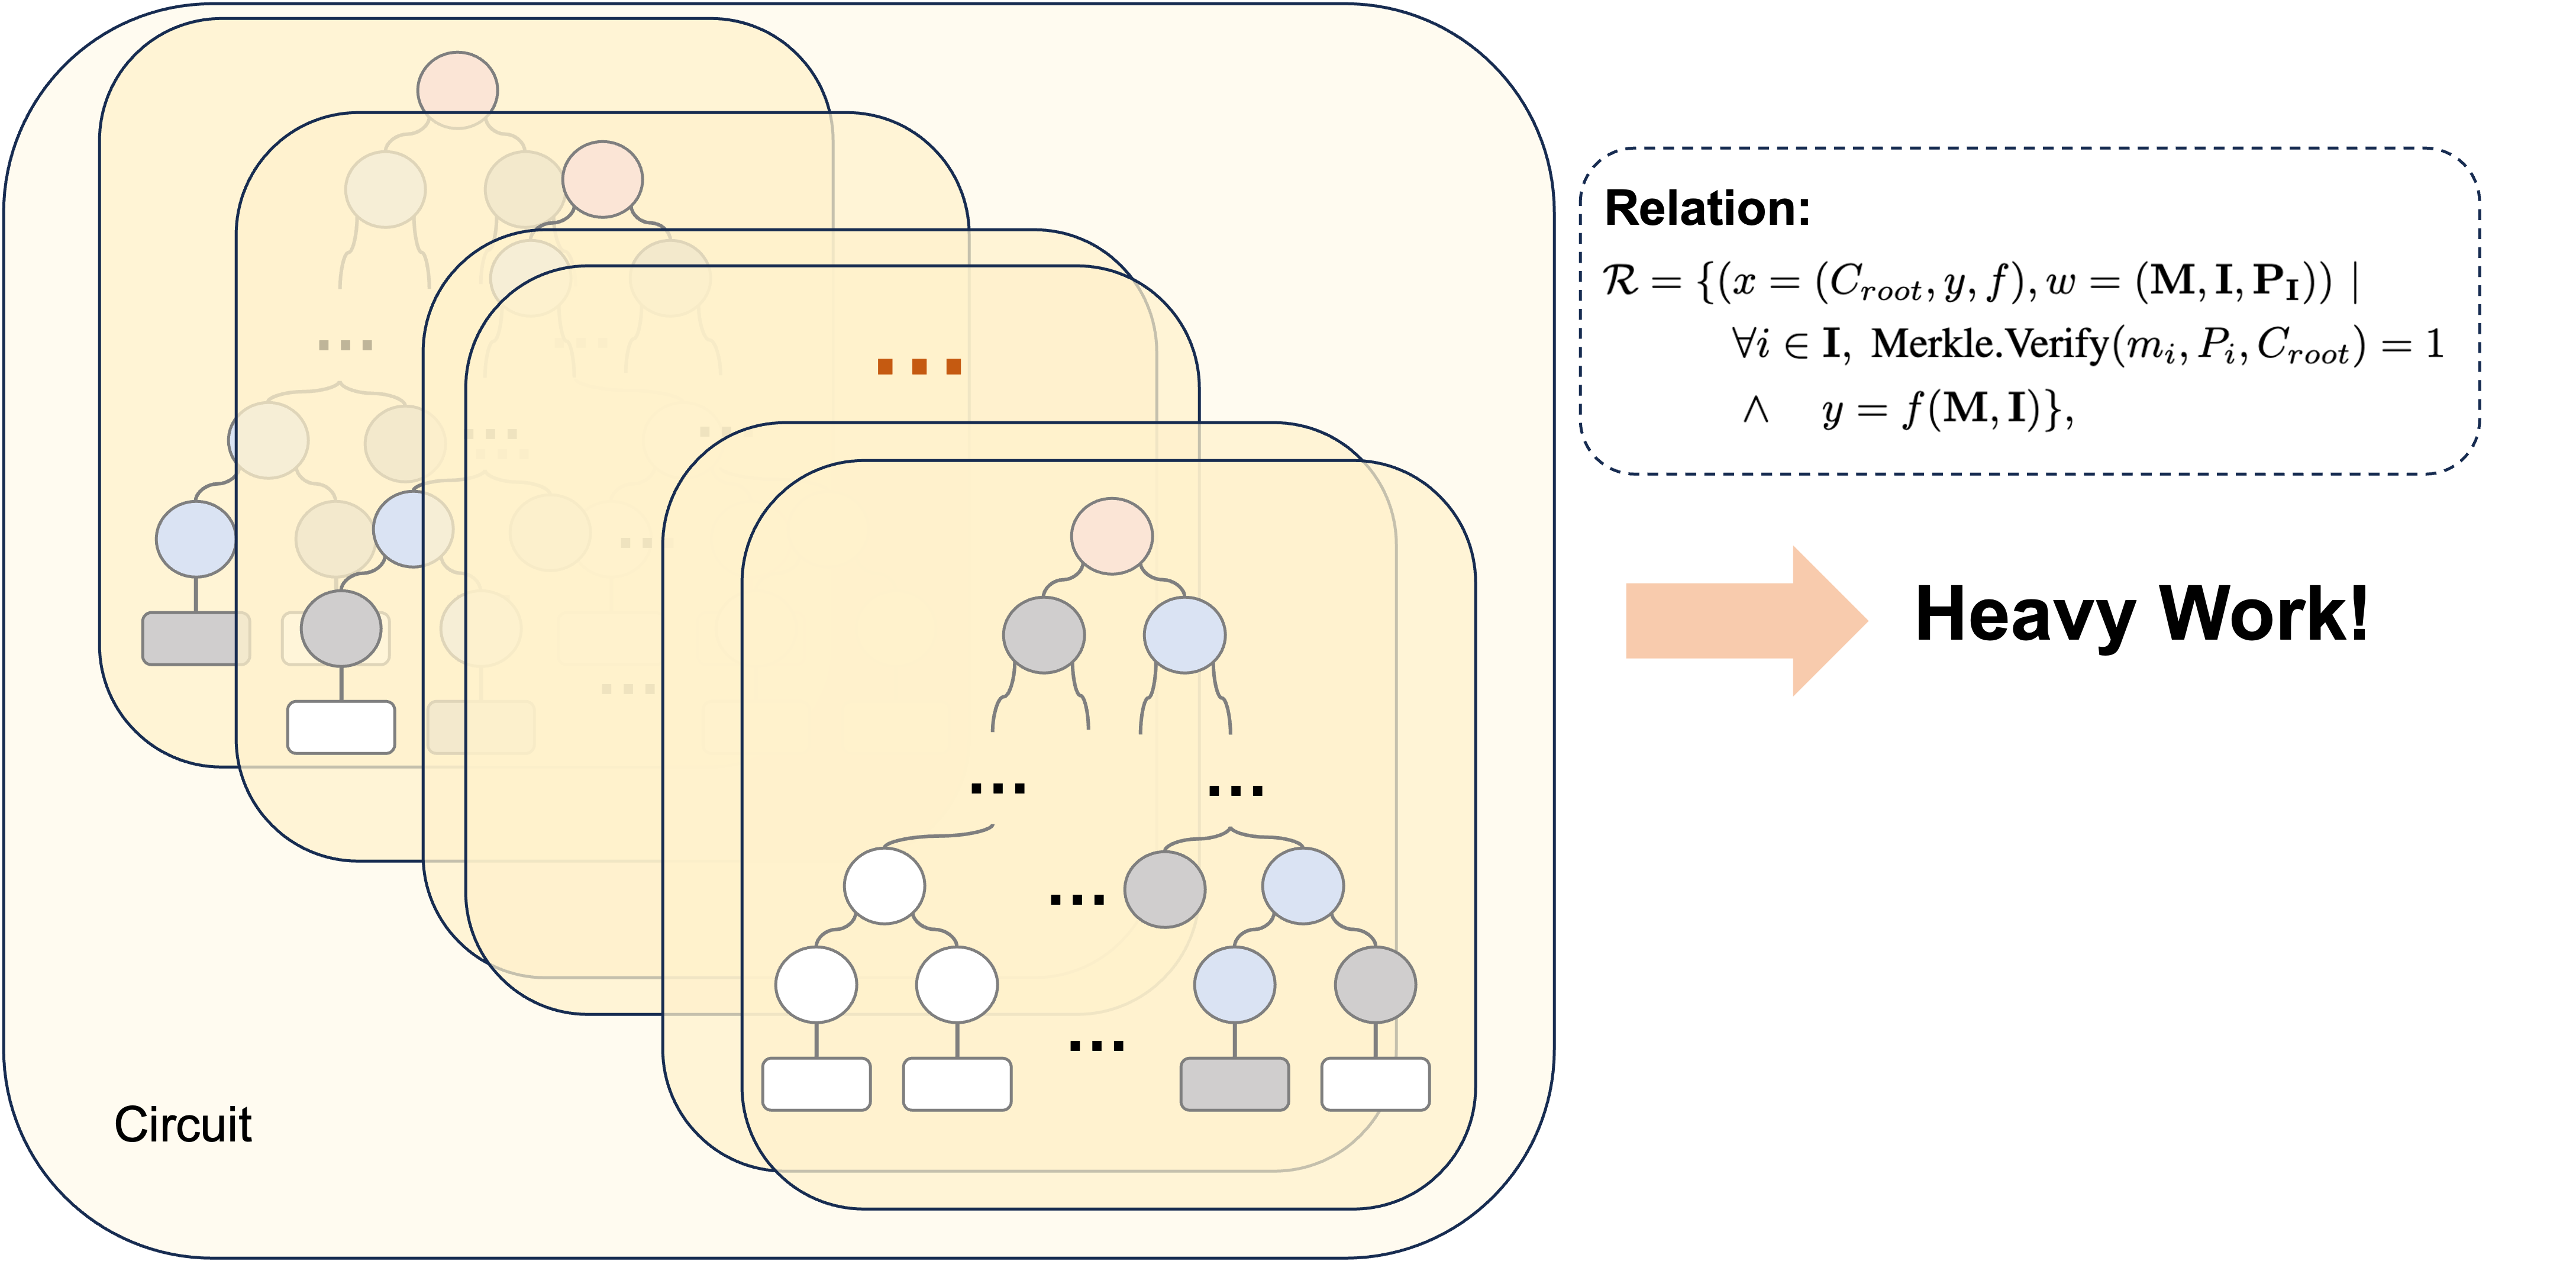
\includegraphics[width=1\linewidth]{44.png}\\

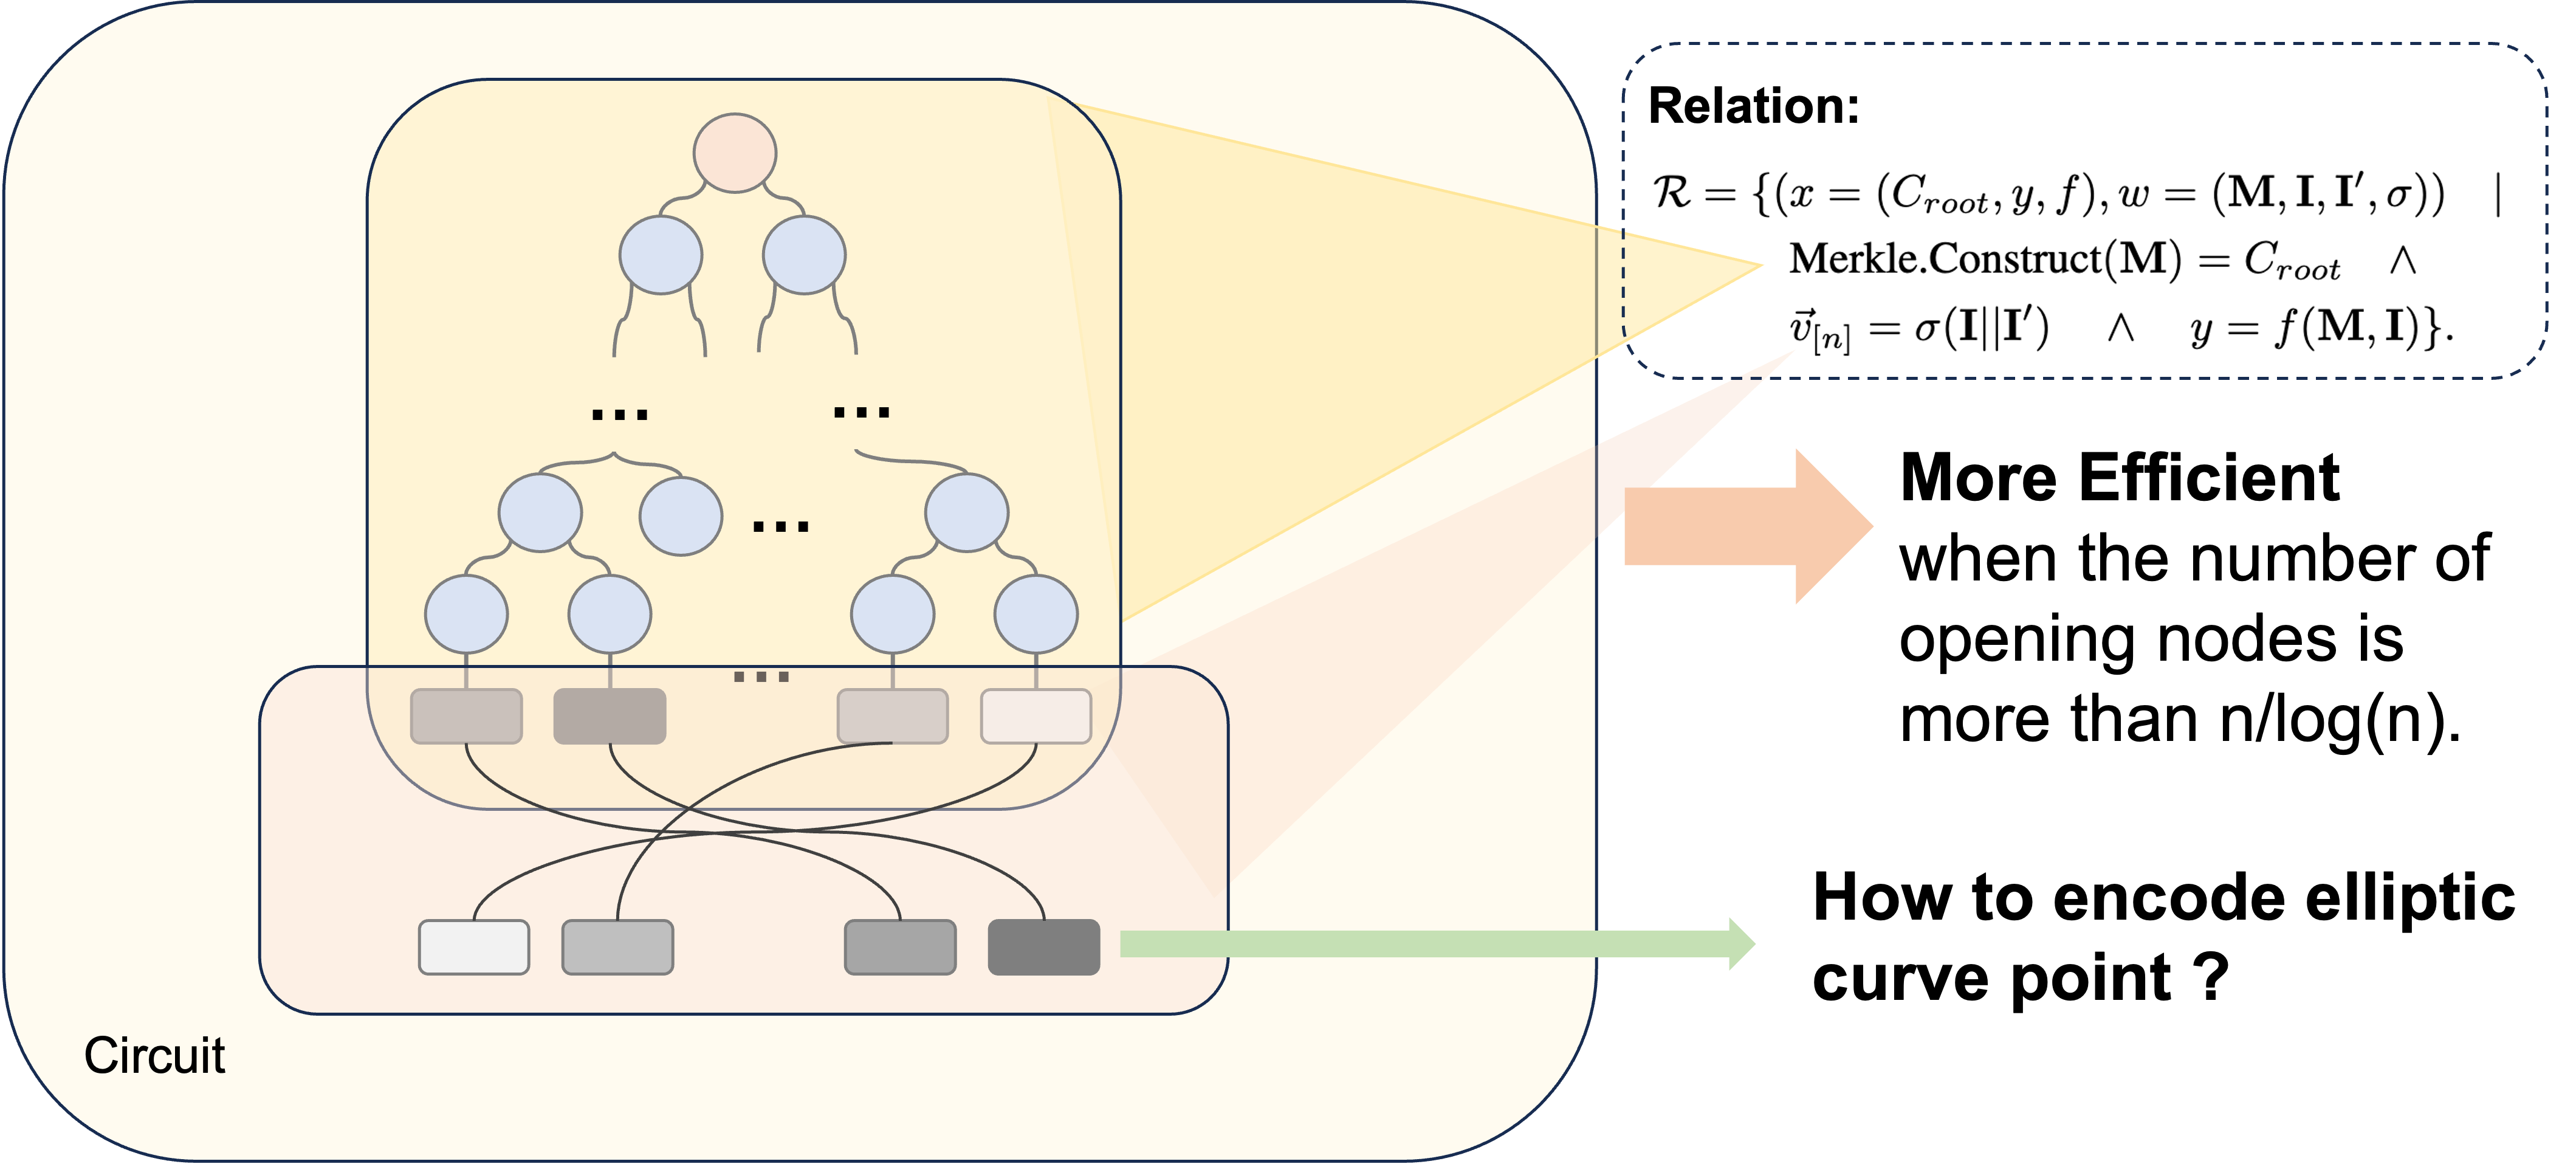
\includegraphics[width=1\linewidth]{55.png}\\


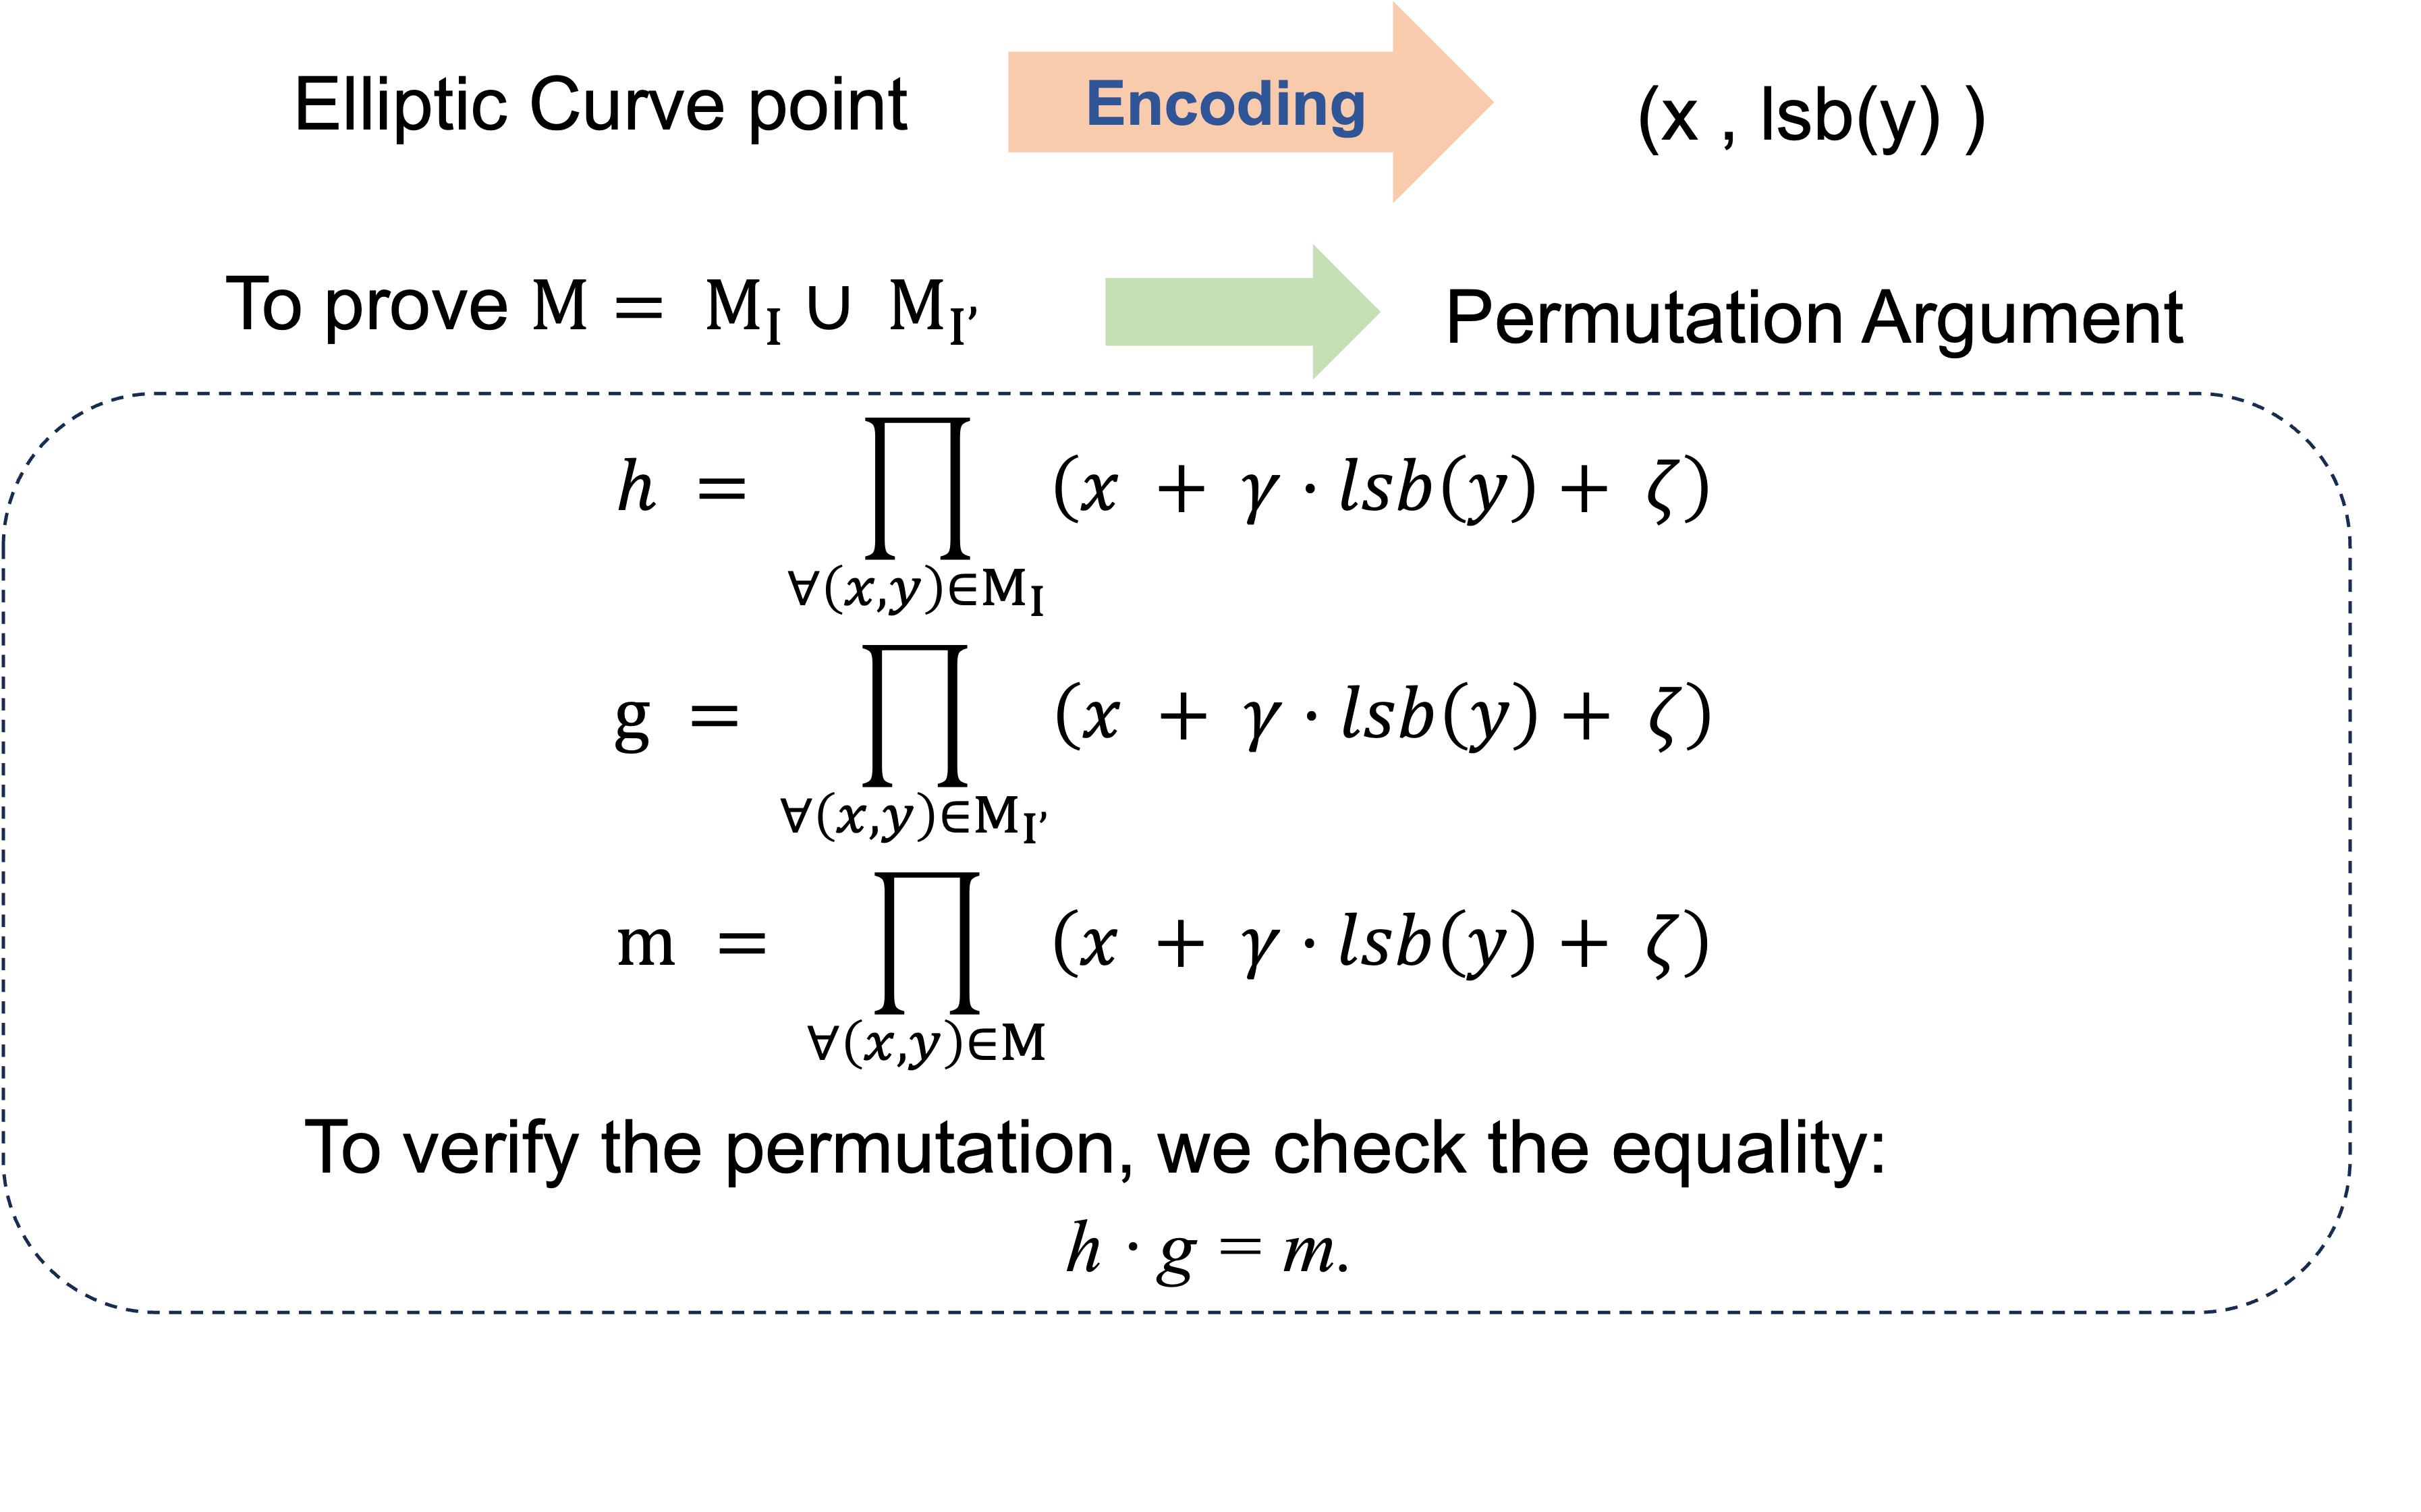
\includegraphics[width=0.9\linewidth]{66.png}

\end{document}
